% Saberes básicos (LOMLOE) asociados a esta unidad
%
% D. La interacción
%   - Predicción de movimientos sencillos a partir de los conceptos de la cinemática, formulando
%     hipótesis comprobables sobre valores futuros de estas magnitudes, validándolas a través del
%     cálculo numérico, la interpretación de gráficas o el trabajo experimental:
%     toda la unidad trabaja posición, distancia, desplazamiento, velocidad y aceleración,
%     tanto a partir de tablas y gráficas posición-tiempo/velocidad-tiempo (MRU y MRUA) como
%     mediante cálculo numérico en ejemplos y ejercicios resueltos.
%   (Las fuerzas, las leyes de Newton y el peso están en la Unidad 8, Las fuerzas.)
%
% A. Las destrezas científicas básicas
%   - Unidades del Sistema Internacional y herramientas matemáticas: uso sistemático de \unit{}
%     y \qty{} (m/s, m/s^2), factores de conversión entre unidades de velocidad, y
%     construcción/interpretación de tablas y gráficas para representar y predecir el movimiento.
%
% (Los bloques B -materia-, C -energía- y E -el cambio- no son objeto de esta unidad.)
%
% (Traducción al español de Unit_7_Motion.tex. Las secciones comentadas del original
%  —caída libre y movimiento circular uniforme— no se traducen; si se recuperan en el libro
%  en inglés, hay que traducirlas aquí también.)

\spacing{1.3}
\raggedbottom % pages with large figures end where the text ends (no stretched gaps between boxes)

\section{Introducción}

Todo lo que nos rodea se mueve: los coches por la carretera, un balón en el patio, la sangre por nuestras venas, la Tierra alrededor del Sol\ldots{} Incluso cuando estás sentado y quieto en clase, ¡te estás moviendo junto con la Tierra! La parte de la física que estudia el movimiento se llama \negsubro{cinemática}.

\begin{definition}[Cinemática]
    Es la parte de la física que estudia el \textbf{movimiento} de los cuerpos: cómo se mueven, con qué rapidez y en qué dirección, \textbf{sin} estudiar las causas de ese movimiento (las fuerzas).
\end{definition}

\begin{definition}[Movimiento]
    Un cuerpo está en \textbf{movimiento} cuando su \textbf{posición cambia} con el tiempo respecto a otro cuerpo que tomamos como referencia. Si su posición no cambia, el cuerpo está \textbf{en reposo}.
\end{definition}

En esta unidad aprenderemos a describir el movimiento con magnitudes como la \textbf{posición}, el \textbf{desplazamiento}, la \textbf{velocidad} y la \textbf{aceleración}, y estudiaremos dos tipos de movimiento sencillos (el movimiento uniforme y el uniformemente acelerado) con tablas, gráficas y fórmulas. En la unidad siguiente, \textbf{Las fuerzas}, veremos con las \textbf{leyes de Newton} cómo cambian las fuerzas el movimiento de los cuerpos.

%----------------------------------------------------------------------------------------

\section{Magnitudes que describen el movimiento}

Para describir un movimiento necesitamos algunas magnitudes básicas. Veámoslas una a una:

\begin{enumerate}[label=\numberballmDarkTeal]
    \item \negsubro{Sistema de referencia}.
    \begin{definition}[Sistema de referencia]
        Es un punto, o un conjunto de puntos, que consideramos fijo y que usamos para describir la posición y el movimiento de otros cuerpos.
    \end{definition}
    \begin{impt}
        \negsubro{El movimiento es relativo}. Que un cuerpo se mueva o no depende del sistema de referencia que elijamos: un cuerpo \textbf{se mueve} si su posición cambia respecto al sistema de referencia, y un mismo cuerpo puede estar en movimiento respecto a un sistema de referencia y en reposo respecto a otro.
    \end{impt}
    \begin{figure}[H]
        \centering
        % [FIGURA ORIGINAL] \includegraphics[width=\textwidth]{Unit_7/reference_frame}
        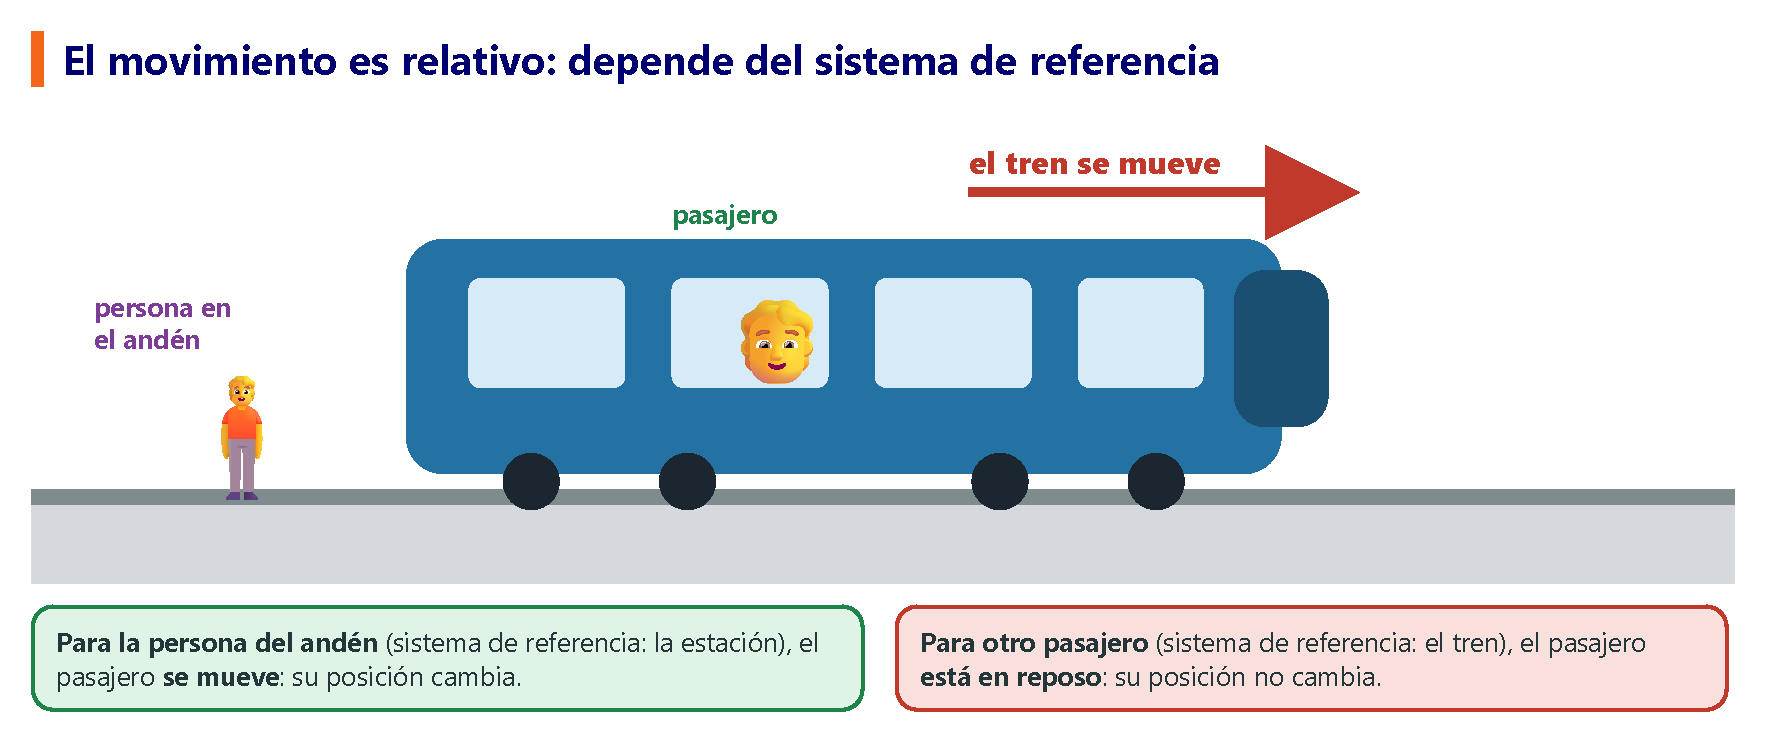
\includegraphics[width=\textwidth]{FigurasSVG/Unit_7_Motion/pdf/reference_frame_es.pdf}
        \caption{Que el pasajero se mueva o no depende del sistema de referencia.}
        \label{fig:u7_reference_frame}
    \end{figure}

    \item \negsubro{Trayectoria}.
    \begin{definition}[Trayectoria]
        Es la línea que sigue un móvil. Puede ser \textbf{rectilínea} (recta), \textbf{circular}, \textbf{parabólica} o de cualquier otra forma.
    \end{definition}

    \item \negsubro{Posición}.
    \begin{definition}[Posición]
        Es el lugar que ocupa un móvil en un instante determinado, medido desde el origen del sistema de referencia. Se representa con la letra \(x\).
    \end{definition}
    La posición \(x\) nos dice \textbf{a qué distancia} está el móvil del origen, así que es una magnitud de \textbf{longitud}: en el SI se mide en \textbf{metros} (\unit{\m}). Escribimos \(x_i\) para la posición \textbf{inicial} y \(x_f\) para la posición \textbf{final}.

    \item \negsubro{Distancia recorrida}.
    \begin{definition}[Distancia recorrida]
        Es la longitud de la trayectoria (el camino) que sigue el móvil.
    \end{definition}

    \item \negsubro{Desplazamiento}.
    \begin{definition}[Desplazamiento]
        Es el cambio de posición de un móvil: su posición final menos su posición inicial. Es la distancia en línea recta entre la posición inicial y la final.
        \begin{equation*}
            \Delta x = x_f - x_i
        \end{equation*}
    \end{definition}
    \begin{itemize}
        \item El símbolo \(\Delta\) (la letra griega \textbf{delta}) significa «\textbf{variación de}»: \(\Delta x\) se lee «delta x» y significa «variación de la posición».
        \item \(x_f\) es la posición \textbf{final} y \(x_i\) la posición \textbf{inicial}. Las dos son posiciones, así que \(\Delta x\) también es una \textbf{longitud} y se mide en \textbf{metros}.
        \item Si \(\Delta x\) es \textbf{positivo}, el móvil se ha alejado del origen (en el sentido positivo); si es \textbf{negativo}, se ha movido en el sentido contrario.
    \end{itemize}
    \begin{figure}[H]
        \centering
        % [FIGURA ORIGINAL] \includegraphics[width=\textwidth]{Unit_7/delta_x_t}
        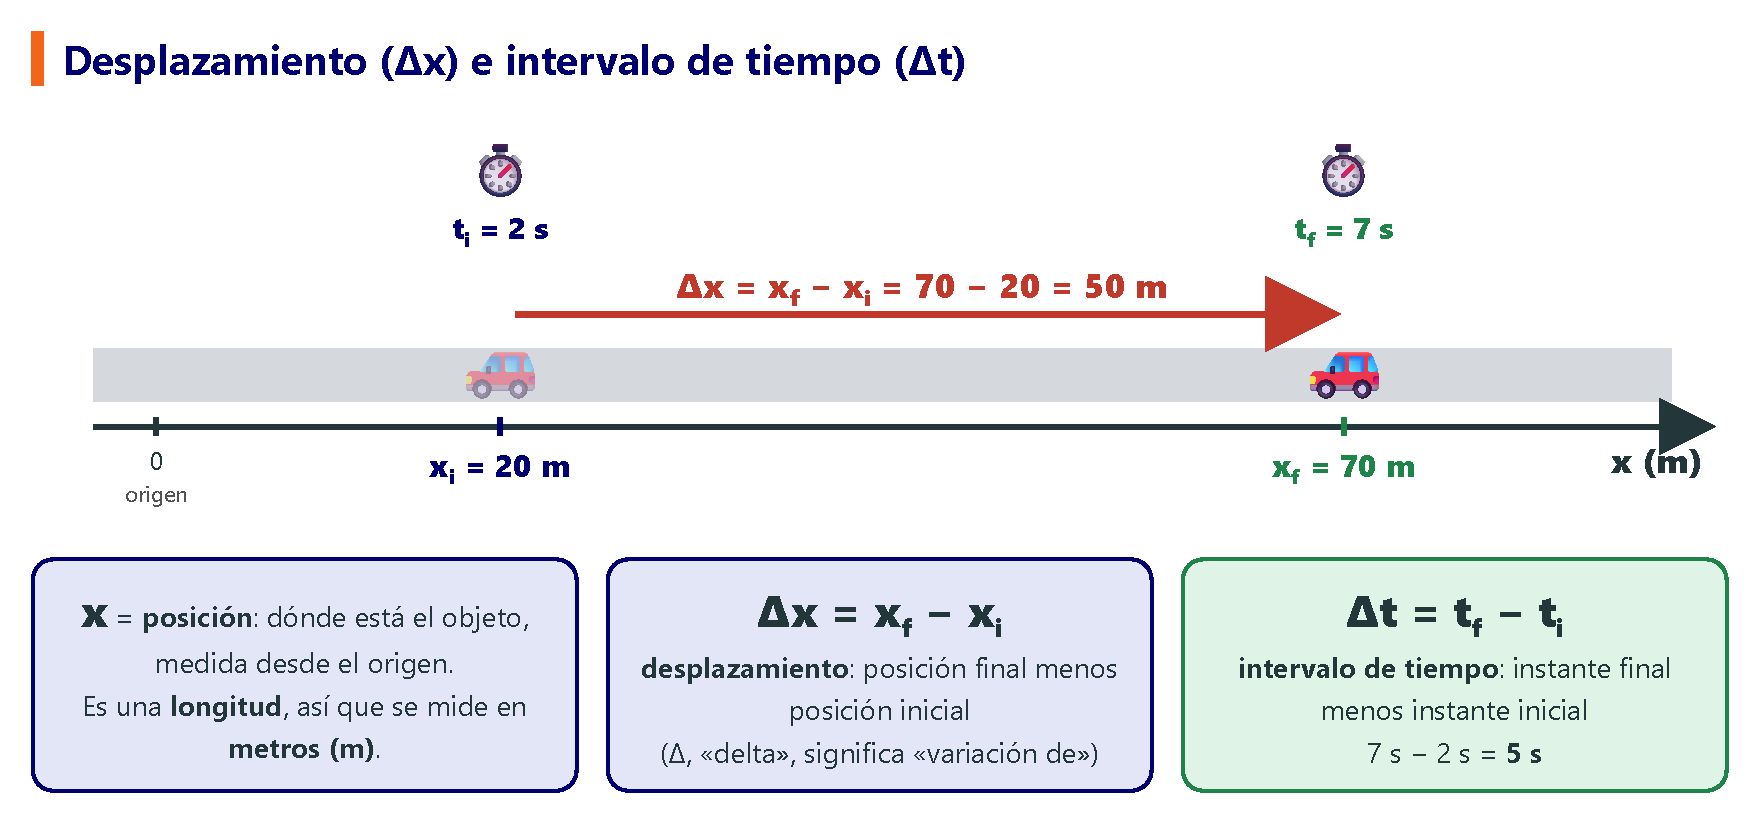
\includegraphics[width=\textwidth]{FigurasSVG/Unit_7_Motion/pdf/delta_x_t_es.pdf}
        \caption{El desplazamiento es la posición final menos la inicial; el intervalo de tiempo es el instante final menos el inicial.}
        \label{fig:u7_delta_x_t}
    \end{figure}
    \begin{figure}[H]
        \centering
        % [FIGURA ORIGINAL] \includegraphics[width=\textwidth]{Unit_7/distance_displacement}
        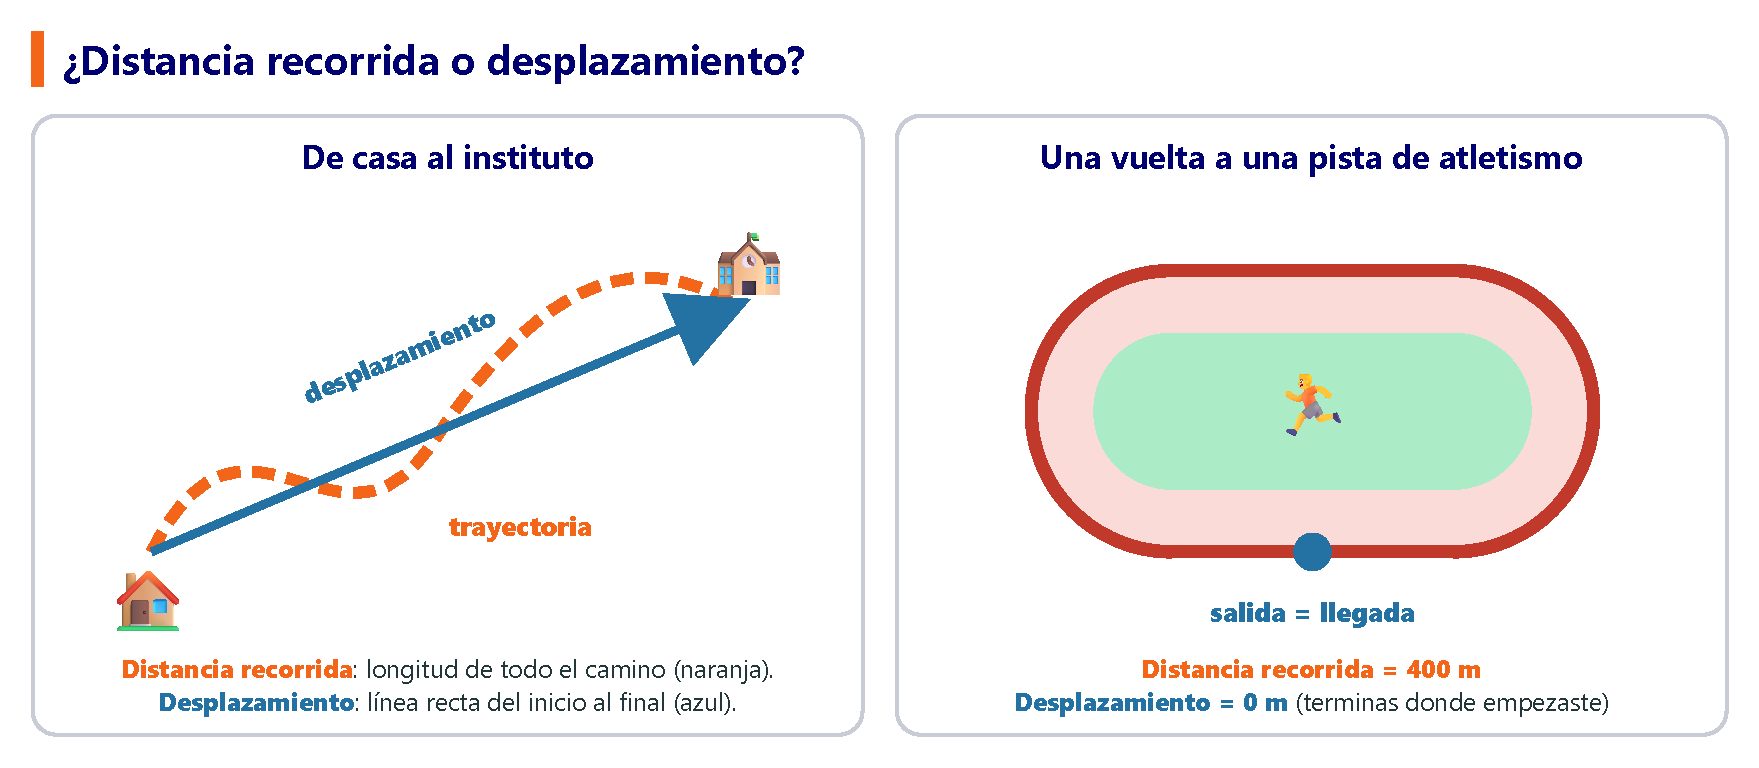
\includegraphics[width=\textwidth]{FigurasSVG/Unit_7_Motion/pdf/distance_displacement_es.pdf}
        \caption{Distancia recorrida (todo el camino) y desplazamiento (la línea recta desde la salida hasta la llegada).}
        \label{fig:u7_distance_displacement}
    \end{figure}
\end{enumerate}

\begin{example}
    \textbf{Un coche está en \(x_i = \qty{20}{\m}\) y, al cabo de un rato, está en \(x_f = \qty{70}{\m}\). Calcula su desplazamiento.}
    \begin{equation*}
        \Delta x = x_f - x_i = \qty{70}{\m} - \qty{20}{\m} = \textcolor{red}{\qty{50}{\m}}
    \end{equation*}
\end{example}

\begin{exercise}
    Una corredora da una vuelta completa a una pista circular de \qty{400}{\m}, saliendo y llegando al mismo punto.
    \begin{enumerate}[label=\letraminuscula]
        \item ¿Qué distancia ha recorrido?
        \item ¿Cuál es su desplazamiento?
    \end{enumerate}
    \begin{solu}
        \begin{enumerate}[label=\alph*)]
            \item Distancia recorrida \(= \qty{400}{\m}\) (la longitud de la vuelta completa).
            \item Desplazamiento \(= \qty{0}{\m}\), porque la posición inicial y la final son el mismo punto.
        \end{enumerate}
    \end{solu}
\end{exercise}

\begin{exercise}
    Dos amigos están sentados en dos autobuses parados, uno al lado del otro. De repente, uno de los autobuses empieza a moverse.
    \begin{enumerate}[label=\letraminuscula]
        \item Explica por qué, al principio, es difícil saber qué autobús se mueve.
        \item Si tomas el otro autobús como sistema de referencia, ¿puedes saber cuál se mueve?
    \end{enumerate}
    \begin{solu}
        \begin{enumerate}[label=\alph*)]
            \item El movimiento es relativo: desde dentro de cada autobús, al principio solo se percibe el movimiento de un autobús respecto al otro, que es igual sea cual sea el que de verdad se mueve.
            \item Sí: si tomas el otro autobús como sistema de referencia fijo, sabes que \emph{tu} autobús se mueve respecto a él en cuanto cambia la distancia entre los dos.
        \end{enumerate}
    \end{solu}
\end{exercise}

\begin{exercise}
    Un ciclista recorre \qty{300}{\m} hacia el norte por una carretera recta, después da la vuelta y recorre \qty{120}{\m} hacia el sur.
    \begin{enumerate}[label=\letraminuscula]
        \item Calcula la distancia recorrida.
        \item Calcula el desplazamiento.
    \end{enumerate}
    \begin{solu}
        \begin{enumerate}[label=\alph*)]
            \item Distancia recorrida \(= \qty{300}{\m} + \qty{120}{\m} = \qty{420}{\m}\) (sumamos todos los metros recorridos, sea cual sea el sentido).
            \item Desplazamiento \(= \qty{300}{\m} - \qty{120}{\m} = \qty{180}{\m}\) hacia el norte (la distancia en línea recta entre el punto de salida y el punto final).
        \end{enumerate}
    \end{solu}
\end{exercise}

\begin{exercise}
    Una senderista camina \qty{2}{\km} hacia el este por un camino recto, después da la vuelta y camina \qty{5}{\km} hacia el oeste.
    \begin{enumerate}[label=\letraminuscula]
        \item Calcula la distancia recorrida.
        \item Calcula el desplazamiento.
    \end{enumerate}
    \begin{solu}
        \begin{enumerate}[label=\alph*)]
            \item Distancia recorrida \(= \qty{2}{\km} + \qty{5}{\km} = \qty{7}{\km}\).
            \item Desplazamiento \(= \qty{5}{\km} - \qty{2}{\km} = \qty{3}{\km}\) hacia el oeste (la distancia en línea recta desde la salida hasta el punto final, en el sentido del tramo más largo).
        \end{enumerate}
    \end{solu}
\end{exercise}

%----------------------------------------------------------------------------------------

\section{La velocidad}

\begin{definition}[Velocidad]
    Es una magnitud que mide lo deprisa que un móvil cambia de posición. Se representa con la letra \(v\) y es el \textbf{desplazamiento} dividido entre el \textbf{intervalo de tiempo}:
    \begin{equation*}
        v = \dfrac{\Delta x}{\Delta t} = \dfrac{x_f - x_i}{t_f - t_i}
    \end{equation*}
    En el SI, la velocidad se mide en \unit{\mps}.
\end{definition}

\begin{itemize}
    \item \(\Delta x = x_f - x_i\) es el \textbf{desplazamiento} (posición final menos posición inicial), en metros.
    \item \(\Delta t = t_f - t_i\) es el \textbf{intervalo de tiempo}: el instante \textbf{final} \(t_f\) menos el instante \textbf{inicial} \(t_i\), en segundos.
\end{itemize}

\begin{impt}
    \negsubro{Cuando no se dice nada más}: si el ejercicio no da la posición inicial ni el instante inicial, tomamos
    \begin{equation*}
        x_i = \qty{0}{\m} \qquad\text{y}\qquad t_i = \qty{0}{\s}
    \end{equation*}
    Entonces \(\Delta x = x_f - 0 = x_f\) y \(\Delta t = t_f - 0 = t_f\). Escribimos simplemente \(x\) en lugar de \(x_f\) y \(t\) en lugar de \(t_f\), y la fórmula de la velocidad queda:
    \begin{equation*}
        v = \dfrac{x}{t}
    \end{equation*}
\end{impt}

\begin{example}
    \textbf{Un coche está en \(x_i = \qty{20}{\m}\) cuando el cronómetro marca \(t_i = \qty{2}{\s}\), y en \(x_f = \qty{70}{\m}\) cuando marca \(t_f = \qty{7}{\s}\). Calcula su velocidad.}
    \begin{equation*}
        v = \dfrac{x_f - x_i}{t_f - t_i} = \dfrac{\qty{70}{\m} - \qty{20}{\m}}{\qty{7}{\s} - \qty{2}{\s}} = \dfrac{\qty{50}{\m}}{\qty{5}{\s}} = \textcolor{red}{\qty{10}{\mps}}
    \end{equation*}
\end{example}

\begin{example}
    \textbf{Una corredora recorre \qty{100}{\m} en \qty{12.5}{\s}. Calcula su velocidad.} No se dice nada de la salida, así que \(x_i = \qty{0}{\m}\) y \(t_i = \qty{0}{\s}\):
    \begin{equation*}
        v = \dfrac{x}{t} = \dfrac{\qty{100}{\m}}{\qty{12.5}{\s}} = \textcolor{red}{\qty{8}{\mps}}
    \end{equation*}
\end{example}

En el lenguaje de todos los días solemos decir \textbf{rapidez} o simplemente velocidad para indicar lo deprisa que se mueve algo. Otras unidades habituales son el \unit{\kmph}, los m/min, las millas por hora o los nudos. Para comparar velocidades dadas en unidades distintas, primero hay que pasarlas a la \textbf{misma} unidad con factores de conversión.

\begin{figure}[H]
    \centering
    % [FIGURA ORIGINAL] \includegraphics[width=\textwidth]{Unit_7/speeds}
    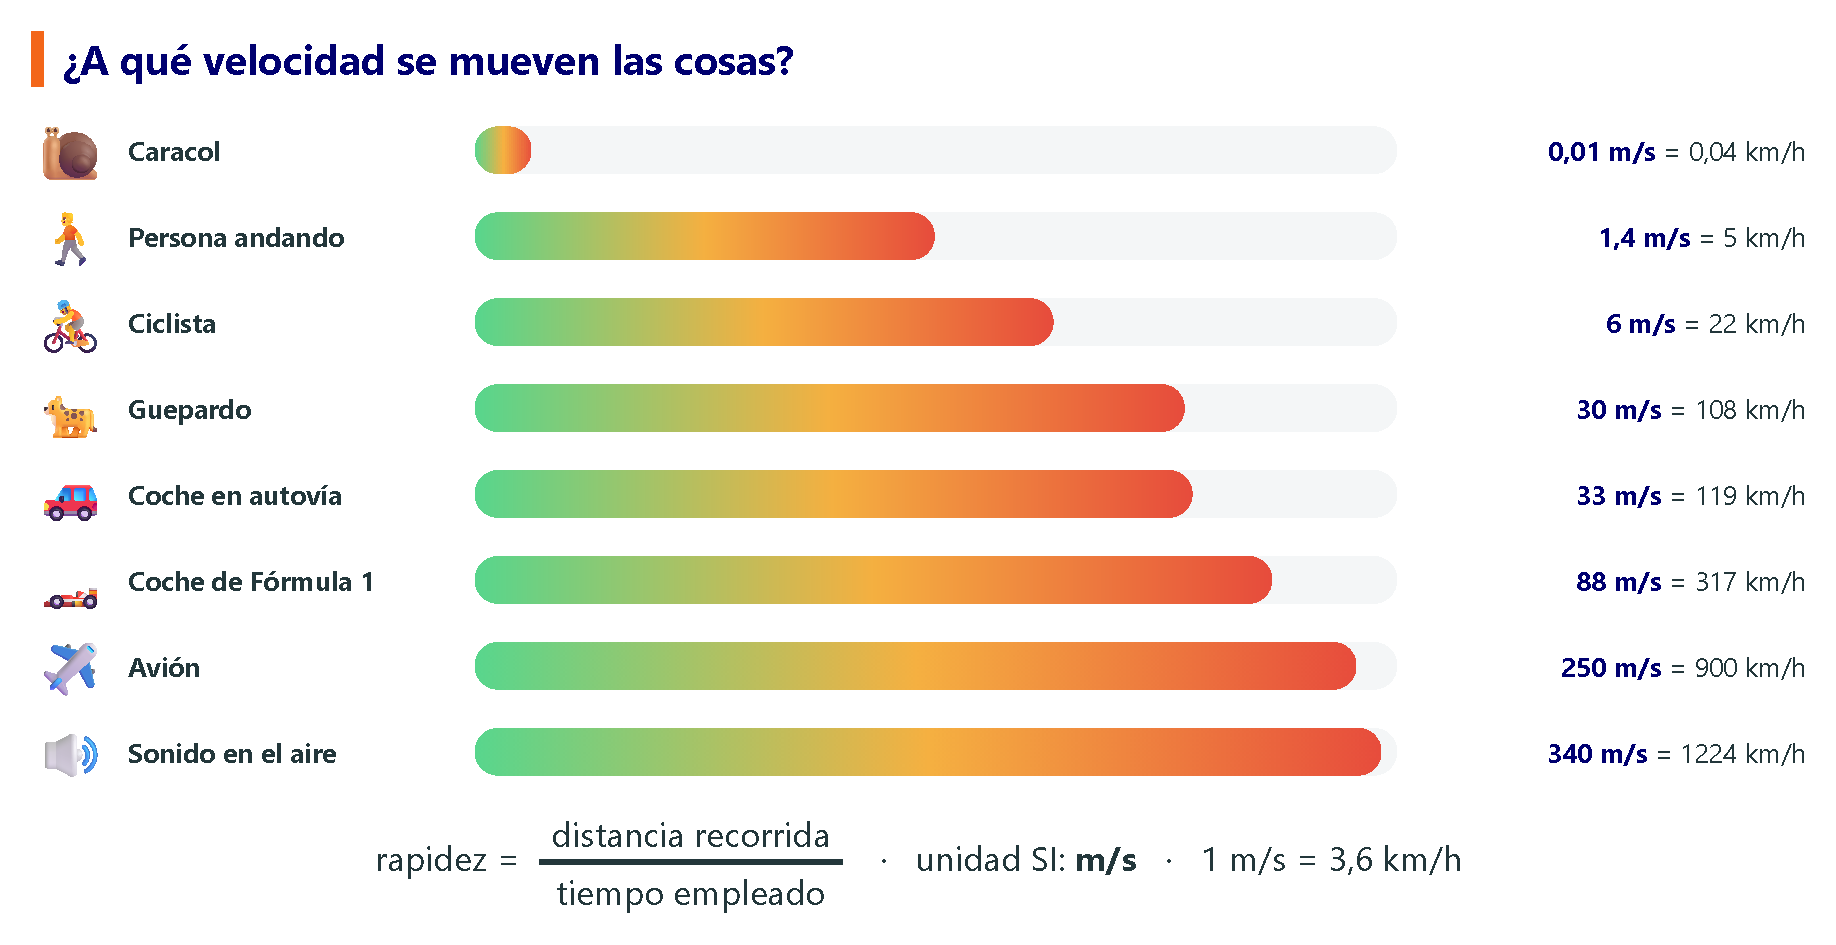
\includegraphics[width=\textwidth]{FigurasSVG/Unit_7_Motion/pdf/speeds_es.pdf}
    \caption{Velocidades de algunos animales, vehículos y del sonido, en m/s y en km/h.}
    \label{fig:u7_speeds}
\end{figure}

\begin{didyouknow}
    Incluso cuando estás sentado y quieto en clase, ¡viajas a unos \qty{107000}{\kmph}! Es la velocidad de la Tierra en su órbita alrededor del Sol. El movimiento es relativo de verdad.
\end{didyouknow}

\begin{example}
    \textbf{Un coche circula a \qty{90}{\kmph} y una moto a \qty{30}{\mps}. ¿Cuál va más deprisa?}
    \begin{equation*}
        90 \dfrac{\text{km}}{\text{h}} \cdot \dfrac{\qty{1000}{\m}}{\qty{1}{\km}} \cdot \dfrac{\qty{1}{\hour}}{\qty{3600}{\s}} = \qty{25}{\mps}
    \end{equation*}
    Como \qty{30}{\mps} \(>\) \qty{25}{\mps}, \textbf{la moto va más deprisa}.
\end{example}

\subsection{Velocidad media y velocidad instantánea}

\begin{itemize}
    \item \negsubro{Velocidad media}: la distancia total recorrida dividida entre el tiempo total empleado en todo el trayecto.
    \item \negsubro{Velocidad instantánea}: la velocidad de un móvil en un instante concreto; es la que marca el velocímetro.
\end{itemize}

\begin{impt}
    La velocidad de un móvil normalmente \textbf{no} es constante durante todo el trayecto, así que su velocidad media suele ser distinta de su velocidad instantánea en un momento dado. Solo pueden coincidir si el móvil va a velocidad constante durante todo el trayecto.
\end{impt}

\begin{example}
    \textbf{Un autobús recorre \qty{1500}{\m} en \qty{150}{\s}. Calcula su velocidad media.}
    \begin{equation*}
        v_{\text{media}} = \dfrac{x}{t} = \dfrac{\qty{1500}{\m}}{\qty{150}{\s}} = \qty{10}{\mps} = \qty{36}{\kmph}
    \end{equation*}
\end{example}

\begin{exercise}
    ¿Qué animal va más deprisa: un ciempiés a \qty{40}{\cm\per\s} o una tortuga a \qty{16.8}{\m\per\minute}?
    \begin{solu}
        Pasamos las dos a la misma unidad, \unit{\cm\per\s}: \\
        Tortuga: \(16.8 \dfrac{\text{m}}{\text{min}} \cdot \dfrac{\qty{100}{\cm}}{\qty{1}{\m}} \cdot \dfrac{\qty{1}{\minute}}{\qty{60}{\s}} = \qty{28}{\cm\per\s}\). \\
        Como \qty{40}{\cm\per\s} \(>\) \qty{28}{\cm\per\s}, \textbf{el ciempiés va más deprisa}.
    \end{solu}
\end{exercise}

\begin{exercise}
    La velocidad de crucero de un avión comercial es de \qty{900}{\kmph}. La velocidad máxima alcanzada en una carrera de Fórmula 1 fue de \qty{88}{\mps}. ¿Cuál es mayor?
    \begin{solu}
        Pasamos la velocidad del avión a \unit{\mps}: \(900 \dfrac{\text{km}}{\text{h}} \cdot \dfrac{\qty{1000}{\m}}{\qty{1}{\km}} \cdot \dfrac{\qty{1}{\hour}}{\qty{3600}{\s}} = \qty{250}{\mps}\). \\
        Como \qty{250}{\mps} \(>\) \qty{88}{\mps}, \textbf{la velocidad de crucero del avión es mayor}.
    \end{solu}
\end{exercise}

\begin{exercise}
    Una camionera recorre los \qty{300}{\km} que separan dos ciudades. Los primeros \qty{200}{\km} los hace a una velocidad media de \qty{100}{\kmph} y, en los \qty{100}{\km} restantes, por el tráfico, su velocidad media baja a \qty{50}{\kmph}.
    \begin{enumerate}[label=\letraminuscula]
        \item Calcula el tiempo que tarda en cada parte del trayecto.
        \item Calcula la velocidad media de todo el trayecto. ¿Es la media de \qty{100}{\kmph} y \qty{50}{\kmph}? Explica por qué sí o por qué no.
    \end{enumerate}
    \begin{solu}
        \begin{enumerate}[label=\alph*)]
            \item \(t_1 = \dfrac{\qty{200}{\km}}{\qty{100}{\kmph}} = \qty{2}{\hour}\); \quad \(t_2 = \dfrac{\qty{100}{\km}}{\qty{50}{\kmph}} = \qty{2}{\hour}\).
            \item Distancia total \(= \qty{300}{\km}\); tiempo total \(= 2 + 2 = \qty{4}{\hour}\). \\
            \(v_{\text{media}} = \dfrac{300}{4} = \qty{75}{\kmph}\). \\
            En este caso concreto \textbf{sí coincide} con la media aritmética de \qty{100}{\kmph} y \qty{50}{\kmph}, porque las dos partes duran \textbf{el mismo tiempo} (\qty{2}{\hour} cada una). En general, la velocidad media \textbf{no} es la media de las velocidades parciales: hay que calcularla siempre como distancia total entre tiempo total.
        \end{enumerate}
    \end{solu}
\end{exercise}

\begin{exercise}
    Un tren recorre los primeros \qty{60}{\km} de un viaje a \qty{120}{\kmph} constantes. Después se para en una estación durante \qty{15}{\minute} y, por último, recorre los \qty{40}{\km} finales a \qty{80}{\kmph} constantes.
    \begin{enumerate}[label=\letraminuscula]
        \item Calcula el tiempo que dura cada una de las tres etapas.
        \item Calcula la velocidad media de todo el viaje (incluida la parada).
    \end{enumerate}
    \begin{solu}
        \begin{enumerate}[label=\alph*)]
            \item \(t_1 = \dfrac{\qty{60}{\km}}{\qty{120}{\kmph}} = \qty{0.5}{\hour}\); \quad \(t_2 = \qty{15}{\minute} = \qty{0.25}{\hour}\); \quad \(t_3 = \dfrac{\qty{40}{\km}}{\qty{80}{\kmph}} = \qty{0.5}{\hour}\).
            \item Distancia total \(= 60 + 40 = \qty{100}{\km}\); tiempo total \(= 0.5 + 0.25 + 0.5 = \qty{1.25}{\hour}\). \\
            \(v_{\text{media}} = \dfrac{100}{1.25} = \qty{80}{\kmph}\).
        \end{enumerate}
    \end{solu}
\end{exercise}

%----------------------------------------------------------------------------------------

\section{Movimiento rectilíneo uniforme (MRU)}

\begin{definition}[Movimiento rectilíneo uniforme (MRU)]
    Es el movimiento de un cuerpo que sigue una trayectoria recta con velocidad \textbf{constante}: recorre la misma distancia en tiempos iguales.
\end{definition}

\subsection{Cálculo de la posición y del tiempo en el MRU}

En el MRU la velocidad es constante, así que podemos usar \(v = \dfrac{x}{t}\) (tomando \(x_i = \qty{0}{\m}\) y \(t_i = \qty{0}{\s}\)) para calcular no solo la velocidad, sino también la \textbf{posición} \(x\) o el \textbf{tiempo} \(t\). Primero tenemos que \textbf{despejar} la magnitud que queremos, igual que hicimos con la densidad en la Unidad 1: una ecuación es como una balanza en equilibrio, y hacemos \textbf{la misma operación en los dos lados}.

\begin{figure}[H]
    \centering
    % [FIGURA ORIGINAL] \includegraphics[width=\textwidth]{Unit_7/velocity_isolate}
    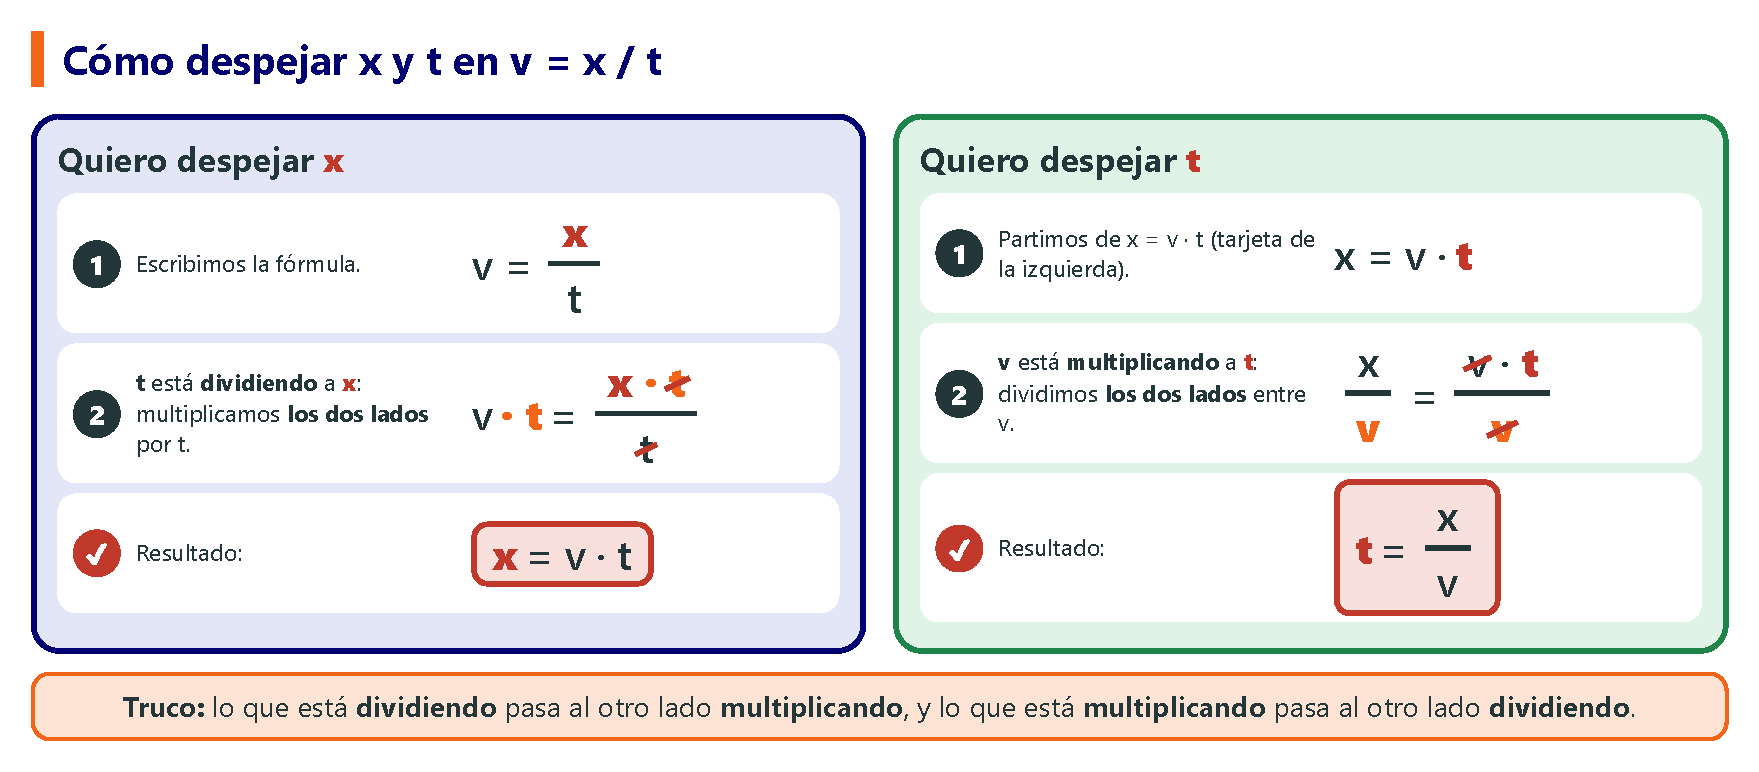
\includegraphics[width=\textwidth]{FigurasSVG/Unit_7_Motion/pdf/velocity_isolate_es.pdf}
    \caption{Cómo despejar la posición \(x\) y el tiempo \(t\) en \(v = x/t\), paso a paso.}
    \label{fig:u7_velocity_isolate}
\end{figure}

\negsubro{Despejar la posición \(x\)}:
\begin{enumerate}[label=\numberballmDarkTeal]
    \item Escribimos la fórmula: \(v = \dfrac{x}{t}\).
    \item \(t\) está \textbf{dividiendo} a \(x\), así que \textbf{multiplicamos los dos lados} por \(t\): \(\;v \cdot t = \dfrac{x \cdot \cancelred{t}}{\cancelred{t}}\).
    \item \(t/t = 1\), así que se simplifica. Damos la vuelta a la ecuación: \(\textcolor{red}{x = v \cdot t}\).
\end{enumerate}

\negsubro{Despejar el tiempo \(t\)}:
\begin{enumerate}[label=\numberballmDarkTeal]
    \item Partimos de \(x = v \cdot t\) (el resultado anterior).
    \item \(v\) está \textbf{multiplicando} a \(t\), así que \textbf{dividimos los dos lados} entre \(v\): \(\;\dfrac{x}{v} = \dfrac{\cancelred{v} \cdot t}{\cancelred{v}}\).
    \item \(v/v = 1\), así que se simplifica. Damos la vuelta a la ecuación: \(\textcolor{red}{t = \dfrac{x}{v}}\).
\end{enumerate}

\begin{impt}
    Las tres versiones de la misma fórmula (con \(x_i = \qty{0}{\m}\) y \(t_i = \qty{0}{\s}\)):
    \begin{equation*}
        v = \dfrac{x}{t} \qquad\qquad x = v \cdot t \qquad\qquad t = \dfrac{x}{v}
    \end{equation*}
    \textbf{Truco}: lo que está \textbf{dividiendo} en un lado pasa al otro lado \textbf{multiplicando}, y lo que está \textbf{multiplicando} pasa al otro lado \textbf{dividiendo}.
\end{impt}

\begin{example}
    \textbf{Cálculo de una posición. Una ciclista va a \qty{6}{\mps} constantes durante \qty{50}{\s}. ¿Dónde está al final, si salió del origen?}
    \begin{enumerate}[label=\numberballmDarkTeal]
        \item Datos: \(v = \qty{6}{\mps}\), \(t = \qty{50}{\s}\), \(x_i = \qty{0}{\m}\). Incógnita: \(\underline{x}\).
        \item Fórmula: \(v = \dfrac{x}{t}\). \(t\) está dividiendo, así que pasa al otro lado multiplicando: \(x = v \cdot t\).
        \item \(x = \qty{6}{\mps} \cdot \qty{50}{\s} = \textcolor{red}{\qty{300}{\m}}\).
    \end{enumerate}
\end{example}

\begin{example}
    \textbf{Cálculo de un tiempo. ¿Cuánto tarda en recorrer \qty{1200}{\m} un caminante que va a \qty{1.5}{\mps} constantes?}
    \begin{enumerate}[label=\numberballmDarkTeal]
        \item Datos: \(v = \qty{1.5}{\mps}\), \(x = \qty{1200}{\m}\). Incógnita: \(\underline{t}\).
        \item Fórmula: \(x = v \cdot t\). \(v\) está multiplicando, así que pasa al otro lado dividiendo: \(t = \dfrac{x}{v}\).
        \item \(t = \dfrac{\qty{1200}{\m}}{\qty{1.5}{\mps}} = \textcolor{red}{\qty{800}{\s}}\) (unos \qty{13.3}{\minute}).
    \end{enumerate}
\end{example}

\begin{exercise}
    Despeja la incógnita y calcula (todos los móviles salen del origen y se mueven con MRU):
    \begin{enumerate}[label=\letraminuscula]
        \item La posición de un coche que circula a \qty{25}{\mps} durante \qty{40}{\s}.
        \item El tiempo que necesita un caracol que se mueve a \qty{0.002}{\mps} para recorrer \qty{1}{\m}.
        \item El tiempo que tarda el sonido en recorrer \qty{1700}{\m} (\(v = \qty{340}{\mps}\)).
        \item La posición de un tren que va a \qty{30}{\mps} al cabo de \qty{2}{\minute} (pasa antes el tiempo a segundos).
    \end{enumerate}
    \begin{solu}
        \begin{enumerate}[label=\alph*)]
            \item \(x = v \cdot t = \qty{25}{\mps} \cdot \qty{40}{\s} = \qty{1000}{\m}\).
            \item \(t = \dfrac{x}{v} = \dfrac{\qty{1}{\m}}{\qty{0.002}{\mps}} = \qty{500}{\s}\).
            \item \(t = \dfrac{x}{v} = \dfrac{\qty{1700}{\m}}{\qty{340}{\mps}} = \qty{5}{\s}\).
            \item \(t = \qty{2}{\minute} = \qty{120}{\s}\); \(x = v \cdot t = \qty{30}{\mps} \cdot \qty{120}{\s} = \qty{3600}{\m}\).
        \end{enumerate}
    \end{solu}
\end{exercise}

\subsection{Gráficas posición-tiempo del MRU}

\begin{figure}[H]
    \centering
    % [FIGURA ORIGINAL] \includegraphics[width=\textwidth]{Unit_7/urm_graphs}
    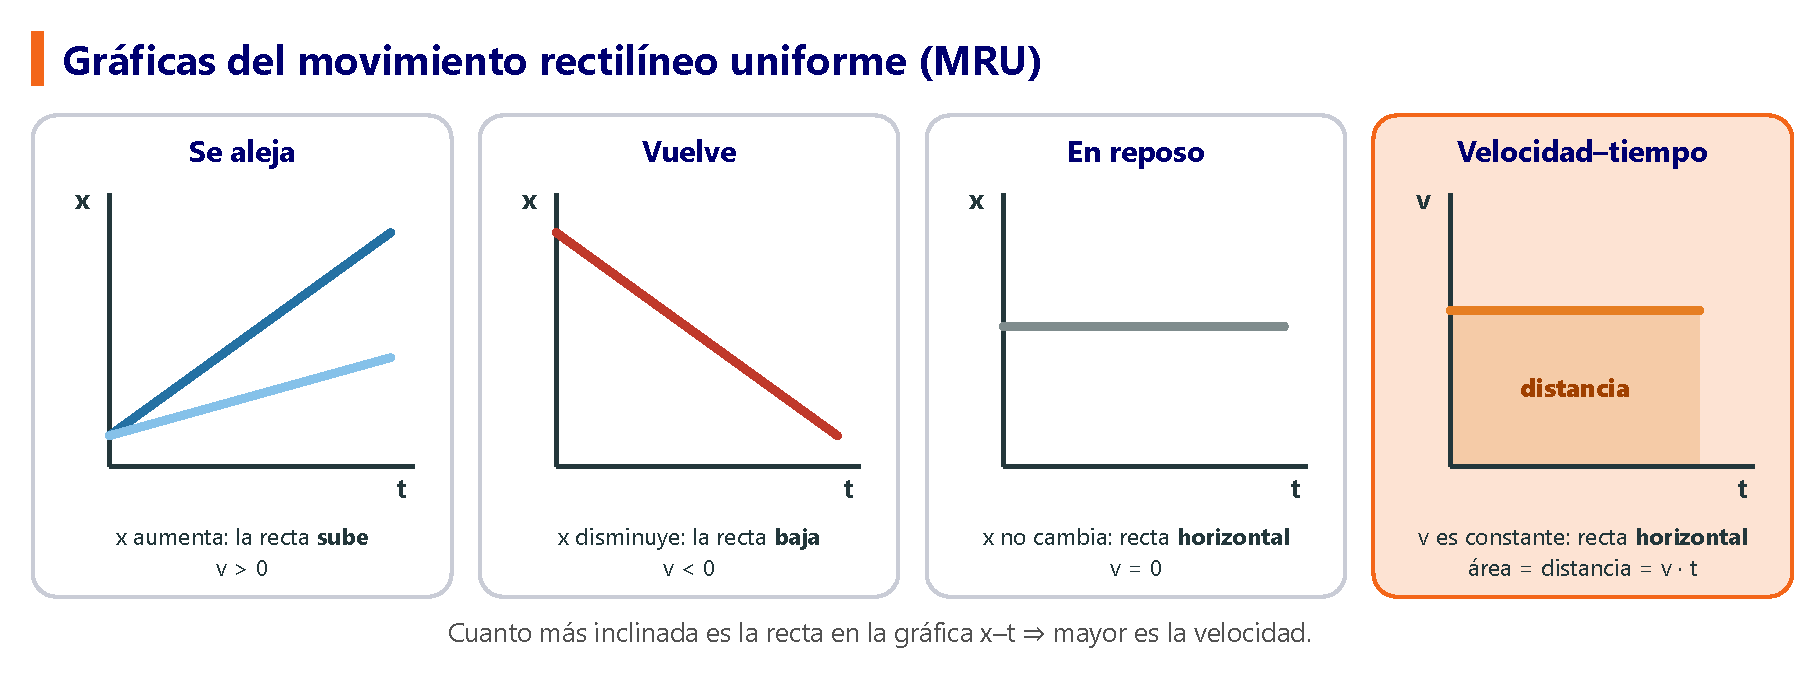
\includegraphics[width=\textwidth]{FigurasSVG/Unit_7_Motion/pdf/urm_graphs_es.pdf}
    \caption{Gráficas posición-tiempo y velocidad-tiempo de un MRU.}
    \label{fig:u7_urm_graphs}
\end{figure}

\begin{itemize}
    \item Si la posición \textbf{aumenta} con el tiempo, la recta sube y el móvil se aleja del origen.
    \item Si la posición \textbf{disminuye} con el tiempo, la recta baja y el móvil se acerca al origen (o lo sobrepasa, hacia posiciones negativas).
    \item La gráfica de un MRU es siempre una \textbf{línea recta}. Cuanto más inclinada está la recta, mayor es la velocidad.
    \item Si la recta pasa por el punto \((0,0)\), el móvil estaba en el origen cuando empezamos a estudiar su movimiento; si no, el móvil ya estaba en otra posición.
\end{itemize}

\begin{impt}
    \negsubro{Lectura de dos rectas de MRU en la misma gráfica}: cuando dibujamos dos rectas posición-tiempo en los mismos ejes, el punto en el que se \textbf{cortan} representa el instante y la posición en los que los dos móviles se encuentran (en ese instante están en el mismo sitio).
\end{impt}

\begin{figure}[H]
    \centering
    % [FIGURA ORIGINAL] \includegraphics[width=0.95\textwidth]{Unit_7/meeting}
    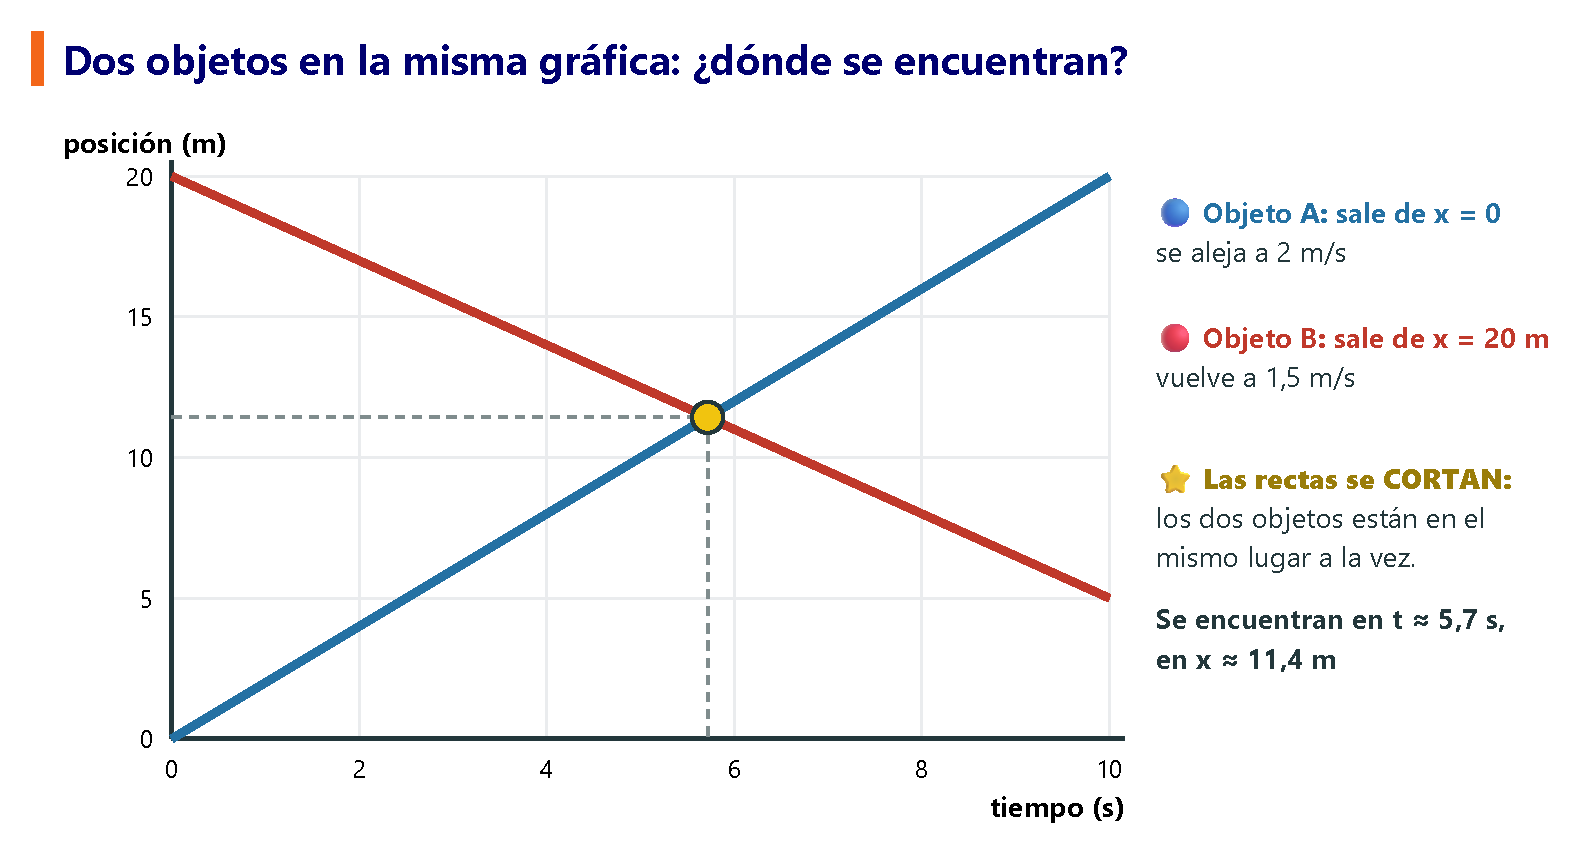
\includegraphics[width=0.95\textwidth]{FigurasSVG/Unit_7_Motion/pdf/meeting_es.pdf}
    \caption{Cuando dos rectas posición-tiempo se cortan, los dos móviles están en el mismo sitio en el mismo instante.}
    \label{fig:u7_meeting}
\end{figure}

\begin{example}
    \textbf{Se registran dos posiciones de un caminante: en \(t=\qty{2}{\s}\), \(x=\qty{3}{\m}\); en \(t=\qty{6}{\s}\), \(x=\qty{11}{\m}\). ¿La gráfica posición-tiempo es creciente o decreciente? ¿Qué nos dice esto sobre el sentido del movimiento?}

    Como \(x\) aumenta de \(\qty{3}{\m}\) a \(\qty{11}{\m}\) al aumentar \(t\), la recta de la gráfica posición-tiempo \textbf{sube}: el caminante se \textbf{aleja} del origen. Con estos dos puntos también podemos calcular la velocidad: \(v = \dfrac{11-3}{6-2} = \qty{2}{\mps}\).
\end{example}

\begin{exercise}
    Una gráfica posición-tiempo muestra una recta horizontal en \(x = \qty{12}{\m}\), desde \(t=0\) hasta \(t=\qty{10}{\s}\).
    \begin{enumerate}[label=\letraminuscula]
        \item ¿Cuál es la velocidad del móvil?
        \item ¿El móvil se mueve respecto al sistema de referencia elegido?
    \end{enumerate}
    \begin{solu}
        \begin{enumerate}[label=\alph*)]
            \item Como la posición no cambia, \(v = \qty{0}{\mps}\).
            \item No: una recta horizontal en una gráfica posición-tiempo significa que el móvil se queda en la misma posición, así que está \textbf{en reposo} respecto a este sistema de referencia.
        \end{enumerate}
    \end{solu}
\end{exercise}

\begin{exercise}
    La gráfica posición-tiempo de un móvil con MRU es una recta que pasa por el origen \((0,0)\) y por el punto \((t,x) = (\qty{5}{\s}, \qty{15}{\m})\).
    \begin{enumerate}[label=\letraminuscula]
        \item ¿Estaba el móvil en el origen en \(t=0\)?
        \item Calcula su velocidad.
        \item Predice su posición en \(t=\qty{8}{\s}\).
    \end{enumerate}
    \begin{solu}
        \begin{enumerate}[label=\alph*)]
            \item Sí: la recta pasa por \((0,0)\), así que el móvil salió del origen.
            \item \(v = \dfrac{\qty{15}{\m} - 0}{\qty{5}{\s} - 0} = \qty{3}{\mps}\).
            \item \(x(8) = v \cdot t = \qty{3}{\mps} \cdot \qty{8}{\s} = \qty{24}{\m}\).
        \end{enumerate}
    \end{solu}
\end{exercise}

\begin{exercise}
    Esta es la gráfica posición-tiempo de un MRU.
    \begin{center}
        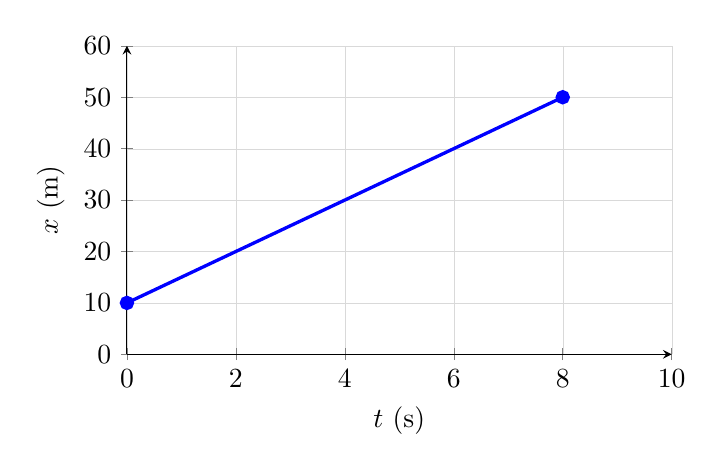
\begin{tikzpicture}
            \begin{axis}[width=8.5cm, height=5.5cm, grid=both, grid style={line width=.1pt, draw=gray!30},
                axis lines=left, xlabel={\(t\) (s)}, ylabel={\(x\) (m)}, xmin=0, xmax=10, ymin=0, ymax=60, xtick={0,2,...,10}, ytick={0,10,...,60}]
                \addplot[very thick, blue, mark=*] coordinates {(0,10) (8,50)};
            \end{axis}
        \end{tikzpicture}
    \end{center}
    \begin{enumerate}[label=\letraminuscula]
        \item ¿Cuál es la posición inicial \(x_i\) del móvil?
        \item Calcula su velocidad usando \(x_i\), \(x_f\), \(t_i\) y \(t_f\).
        \item ¿El móvil se aleja del origen o se acerca a él?
        \item Lee en la gráfica la posición en \(t = \qty{4}{\s}\) y compruébala con un cálculo.
    \end{enumerate}
    \begin{solu}
        \begin{enumerate}[label=\alph*)]
            \item En \(t = \qty{0}{\s}\) la recta empieza en \(x_i = \qty{10}{\m}\): el móvil no salió del origen.
            \item \(v = \dfrac{x_f - x_i}{t_f - t_i} = \dfrac{\qty{50}{\m} - \qty{10}{\m}}{\qty{8}{\s} - \qty{0}{\s}} = \qty{5}{\mps}\).
            \item La recta sube (\(v > 0\)): se \textbf{aleja} del origen.
            \item En la gráfica, \(x = \qty{30}{\m}\). Cálculo: \(x = x_i + v \cdot t = \qty{10}{\m} + \qty{5}{\mps} \cdot \qty{4}{\s} = \qty{30}{\m}\).
        \end{enumerate}
    \end{solu}
\end{exercise}

\begin{exercise}
    La gráfica muestra la posición de un alumno que camina por un pasillo recto.
    \begin{center}
        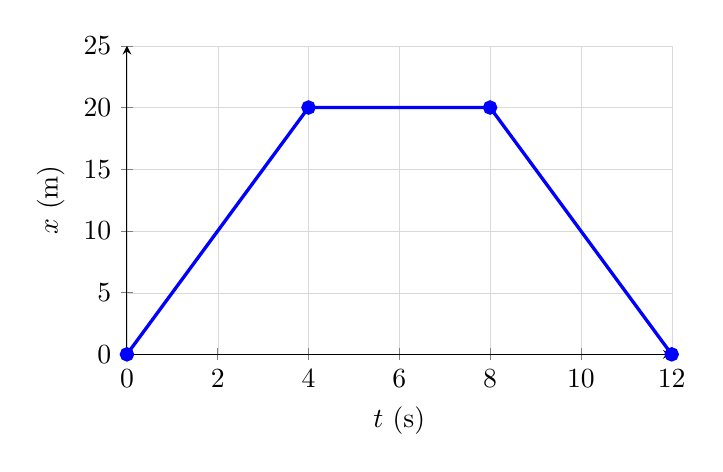
\begin{tikzpicture}
            \begin{axis}[width=8.5cm, height=5.5cm, grid=both, grid style={line width=.1pt, draw=gray!30},
                axis lines=left, xlabel={\(t\) (s)}, ylabel={\(x\) (m)}, xmin=0, xmax=12, ymin=0, ymax=25, xtick={0,2,...,12}, ytick={0,5,...,25}]
                \addplot[very thick, blue, mark=*] coordinates {(0,0) (4,20) (8,20) (12,0)};
            \end{axis}
        \end{tikzpicture}
    \end{center}
    \begin{enumerate}[label=\letraminuscula]
        \item Describe lo que hace el alumno en cada tramo: \(0\)--\(4\) s, \(4\)--\(8\) s y \(8\)--\(12\) s.
        \item Calcula la velocidad en cada tramo.
        \item Calcula la distancia total recorrida y el desplazamiento total.
    \end{enumerate}
    \begin{solu}
        \begin{enumerate}[label=\alph*)]
            \item \(0\)--\(4\) s: se aleja del origen. \(4\)--\(8\) s: se queda en \(x = \qty{20}{\m}\) (en reposo). \(8\)--\(12\) s: vuelve al origen.
            \item \(v_1 = \dfrac{20 - 0}{4 - 0} = \qty{5}{\mps}\); \quad \(v_2 = \dfrac{20 - 20}{8 - 4} = \qty{0}{\mps}\); \quad \(v_3 = \dfrac{0 - 20}{12 - 8} = \qty{-5}{\mps}\).
            \item Distancia recorrida \(= \qty{20}{\m} + \qty{0}{\m} + \qty{20}{\m} = \qty{40}{\m}\). Desplazamiento \(\Delta x = x_f - x_i = \qty{0}{\m} - \qty{0}{\m} = \qty{0}{\m}\) (termina donde empezó).
        \end{enumerate}
    \end{solu}
\end{exercise}

\begin{exercise}
    La gráfica muestra las posiciones de dos coches, \(A\) y \(B\), que se mueven por la misma carretera recta.
    \begin{center}
        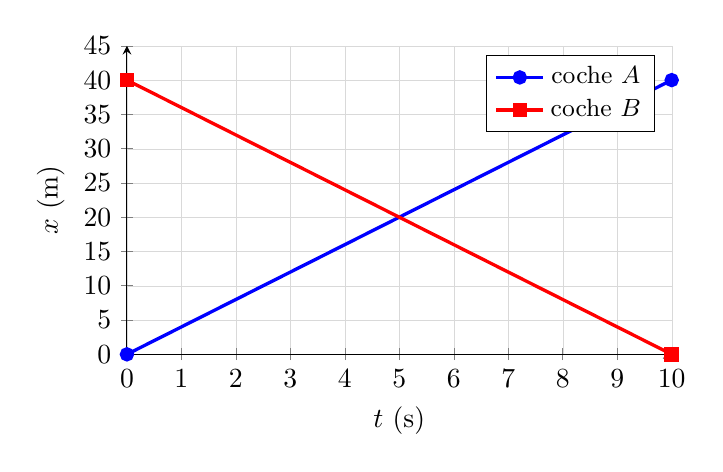
\begin{tikzpicture}
            \begin{axis}[width=8.5cm, height=5.5cm, grid=both, grid style={line width=.1pt, draw=gray!30},
                axis lines=left, xlabel={\(t\) (s)}, ylabel={\(x\) (m)}, xmin=0, xmax=10, ymin=0, ymax=45, xtick={0,1,...,10}, ytick={0,5,...,45}, legend pos=north east, legend style={font=\small}]
                \addplot[very thick, blue, mark=*] coordinates {(0,0) (10,40)};
                \addlegendentry{coche \(A\)}
                \addplot[very thick, red, mark=square*] coordinates {(0,40) (10,0)};
                \addlegendentry{coche \(B\)}
            \end{axis}
        \end{tikzpicture}
    \end{center}
    \begin{enumerate}[label=\letraminuscula]
        \item Calcula la velocidad de cada coche. ¿Qué significa el signo de cada velocidad?
        \item ¿En qué instante y en qué posición se encuentran los dos coches?
    \end{enumerate}
    \begin{solu}
        \begin{enumerate}[label=\alph*)]
            \item \(v_A = \dfrac{40 - 0}{10 - 0} = \qty{4}{\mps}\) (positiva: se aleja del origen). \(v_B = \dfrac{0 - 40}{10 - 0} = \qty{-4}{\mps}\) (negativa: se acerca al origen).
            \item Las rectas se cortan en \(t = \qty{5}{\s}\) y \(x = \qty{20}{\m}\): ahí se encuentran los dos coches.
        \end{enumerate}
    \end{solu}
\end{exercise}

\begin{exercise}
    Un coche de juguete se mueve con MRU. Sus posiciones se recogen en esta tabla:
    \begin{center}
        \begin{tabular}{lcccccc}
            \toprule
            \(t\) (s) & 0 & 1 & 2 & 3 & 4 & 5 \\
            \midrule
            \(x\) (m) & 0 & 3 & 6 & 9 & 12 & 15 \\
            \bottomrule
        \end{tabular}
    \end{center}
    \begin{enumerate}[label=\letraminuscula]
        \item Dibuja la gráfica posición-tiempo (\(t\) en el eje horizontal y \(x\) en el eje vertical).
        \item ¿Qué forma tiene la gráfica? ¿Por qué?
        \item Calcula la velocidad del coche.
    \end{enumerate}
    \begin{solu}
        \begin{enumerate}[label=\alph*)]
            \item Los puntos \((0,0)\), \((1,3)\), \((2,6)\), \((3,9)\), \((4,12)\) y \((5,15)\) se unen con una línea recta.
    \begin{center}
                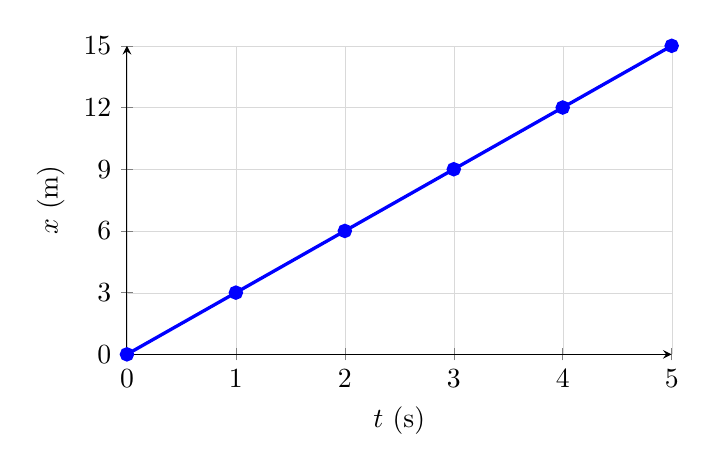
\begin{tikzpicture}
                    \begin{axis}[width=8.5cm, height=5.5cm, grid=both, grid style={line width=.1pt, draw=gray!30},
                        axis lines=left, xlabel={\(t\) (s)}, ylabel={\(x\) (m)}, xmin=0, xmax=5, ymin=0, ymax=15, xtick={0,1,...,5}, ytick={0,3,...,15}]
                        \addplot[very thick, blue, mark=*] coordinates {(0,0) (1,3) (2,6) (3,9) (4,12) (5,15)};
                    \end{axis}
                \end{tikzpicture}
            \end{center}
            \item Una recta que sube y pasa por el origen, porque el coche recorre la misma distancia (\qty{3}{\m}) cada segundo: su velocidad es constante.
            \item \(v = \dfrac{x_f - x_i}{t_f - t_i} = \dfrac{\qty{15}{\m} - \qty{0}{\m}}{\qty{5}{\s} - \qty{0}{\s}} = \qty{3}{\mps}\).
        \end{enumerate}
    \end{solu}
\end{exercise}

\subsection{Velocidad de un MRU a partir de una tabla o de una gráfica}

Para calcular la velocidad de un MRU, toma dos puntos cualesquiera \(A\) y \(B\) de una tabla o de una gráfica. El punto \(A\) es el \textbf{inicial} y el punto \(B\) el \textbf{final}:
\begin{equation*}
    x_A = x_i \qquad t_A = t_i \qquad\qquad x_B = x_f \qquad t_B = t_f
\end{equation*}
Así que la fórmula es exactamente la misma fórmula de la velocidad que ya conocemos:
\begin{equation*}
    v = \dfrac{x_B - x_A}{t_B - t_A} = \dfrac{x_f - x_i}{t_f - t_i} = \dfrac{\Delta x}{\Delta t}
\end{equation*}

\begin{example}
    \textbf{Un punto \(A\) está en \(x = \qty{10}{\m}\) cuando \(t = \qty{4}{\s}\); un punto \(B\) está en \(x = \qty{30}{\m}\) cuando \(t = \qty{12}{\s}\). Calcula la velocidad.} \\
    El punto \(A\) es el inicial: \(x_i = \qty{10}{\m}\), \(t_i = \qty{4}{\s}\). El punto \(B\) es el final: \(x_f = \qty{30}{\m}\), \(t_f = \qty{12}{\s}\).
    \begin{equation*}
        v = \dfrac{\qty{30}{\m} - \qty{10}{\m}}{\qty{12}{\s} - \qty{4}{\s}} = \qty{2.5}{\mps}
    \end{equation*}
    Una velocidad \textbf{positiva} significa que el móvil se aleja del origen.
\end{example}

\begin{impt}
    Si, en cambio, la posición \textbf{disminuye} entre los dos puntos, la velocidad sale \textbf{negativa}. Esto significa que el móvil se acerca al origen (o lo sobrepasa).
\end{impt}

\begin{exercise}
    Un punto \(A\) está en \(x = \qty{50}{\m}\) cuando \(t = \qty{5}{\s}\); un punto \(B\) está en \(x = \qty{20}{\m}\) cuando \(t = \qty{15}{\s}\).
    \begin{enumerate}[label=\letraminuscula]
        \item Calcula la velocidad.
        \item ¿Qué te dice el signo de la velocidad sobre el sentido del movimiento?
    \end{enumerate}
    \begin{solu}
        \begin{enumerate}[label=\alph*)]
            \item \(v = \dfrac{\qty{20}{\m} - \qty{50}{\m}}{\qty{15}{\s} - \qty{5}{\s}} = \qty{-3}{\mps}\).
            \item La velocidad es \textbf{negativa}, así que el móvil se acerca al origen (su posición disminuye con el tiempo).
        \end{enumerate}
    \end{solu}
\end{exercise}

\begin{exercise}
    La tabla muestra la posición de un tren de juguete cada \qty{3}{\s}:
    \begin{center}
        \begin{tabular}{lcccc}
            \toprule
            Tiempo (s) & 0 & 3 & 6 & 9 \\
            \midrule
            Posición (m) & 2 & 14 & 26 & 38 \\
            \bottomrule
        \end{tabular}
    \end{center}
    \begin{enumerate}[label=\letraminuscula]
        \item Calcula la velocidad con los dos primeros puntos de la tabla.
        \item Comprueba, con otra pareja de puntos, que el movimiento es de verdad un MRU.
        \item Predice la posición del tren en \(t=\qty{12}{\s}\).
    \end{enumerate}
    \begin{solu}
        \begin{enumerate}[label=\alph*)]
            \item \(v = \dfrac{\qty{14}{\m} - \qty{2}{\m}}{\qty{3}{\s} - \qty{0}{\s}} = \qty{4}{\mps}\).
            \item Entre \(t=6\) s y \(t=9\) s: \(v = \dfrac{38-26}{9-6} = \qty{4}{\mps}\), el mismo valor, así que la velocidad es constante: se confirma que es un MRU.
            \item \(x(12) = x(0) + v \cdot t = \qty{2}{\m} + \qty{4}{\mps} \cdot \qty{12}{\s} = \qty{50}{\m}\).
        \end{enumerate}
    \end{solu}
\end{exercise}

\subsection{Gráficas velocidad-tiempo del MRU}

Como la velocidad de un MRU es constante, su gráfica velocidad-tiempo es siempre una \textbf{recta horizontal}.

\begin{impt}
    \negsubro{Distancia recorrida a partir de una gráfica velocidad-tiempo}: la distancia recorrida es igual al \textbf{área} comprendida entre la recta velocidad-tiempo y el eje del tiempo. En un MRU esa área es un rectángulo: \(\text{distancia} = v \cdot t\), que es la misma ecuación que ya usamos para calcular la velocidad.
\end{impt}

\begin{example}
    \textbf{Un ciclista va a \qty{4}{\mps} constantes durante \qty{15}{\s}. Calcula la distancia recorrida usando el área bajo la gráfica velocidad-tiempo.}

    La gráfica velocidad-tiempo es una recta horizontal en \(v = \qty{4}{\mps}\), entre \(t=0\) y \(t=\qty{15}{\s}\). El área que queda debajo es un rectángulo:
    \begin{equation*}
        \text{distancia} = v \cdot t = \qty{4}{\mps} \cdot \qty{15}{\s} = \qty{60}{\m}
    \end{equation*}
\end{example}

\begin{exercise}
    La tabla muestra la posición de un coche teledirigido cada \qty{10}{\s}:
    \begin{center}
        \begin{tabular}{lcccc}
            \toprule
            Tiempo (s) & 0 & 10 & 20 & 30 \\
            \midrule
            Posición (m) & 10 & 30 & 30 & 0 \\
            \bottomrule
        \end{tabular}
    \end{center}
    \begin{enumerate}[label=\letraminuscula]
        \item Calcula la velocidad en cada tramo del recorrido.
        \item Calcula la velocidad media de todo el recorrido.
    \end{enumerate}
    \begin{solu}
        \begin{enumerate}[label=\alph*)]
            \item Tramo 1 (de \(t=0\) a \(10\) s): \(v_1 = \dfrac{30-10}{10-0} = \qty{2}{\mps}\). \\
            Tramo 2 (de \(t=10\) a \(20\) s): la posición no cambia, así que \(v_2 = \qty{0}{\mps}\) (el coche está en reposo). \\
            Tramo 3 (de \(t=20\) a \(30\) s): \(v_3 = \dfrac{0-30}{30-20} = \qty{-3}{\mps}\) (se acerca al origen).
            \item Distancia total recorrida \(= \qty{20}{\m} + \qty{0}{\m} + \qty{30}{\m} = \qty{50}{\m}\); tiempo total \(= \qty{30}{\s}\). \\
            \(v_{\text{media}} = \dfrac{50}{30} \approx \qty{1.67}{\mps}\).
        \end{enumerate}
    \end{solu}
\end{exercise}

\begin{exercise}
    Una ciclista pasa por el punto kilométrico \qty{20}{\km} cuando se pone en marcha el cronómetro, y va a velocidad constante. Llega al punto kilométrico \qty{40}{\km} a los \qty{25}{\minute}, se para a descansar \qty{20}{\minute} y después recorre los \qty{20}{\km} siguientes en \qty{10}{\minute}, de nuevo a velocidad constante.
    \begin{enumerate}[label=\letraminuscula]
        \item Calcula su velocidad en cada uno de los tres tramos.
        \item Calcula su velocidad media en todo el recorrido.
    \end{enumerate}
    \begin{solu}
        \begin{enumerate}[label=\alph*)]
            \item Tramo 1: \(v_1 = \dfrac{40\qty{-20}{\km}}{25\qty{-0}{\minute}} = \qty{0.8}{\km\per\minute}\). \\
            Tramo 2 (descansando): \(v_2 = \qty{0}{\km\per\minute}\). \\
            Tramo 3: \(v_3 = \dfrac{60\qty{-40}{\km}}{55\qty{-45}{\minute}} = \qty{2}{\km\per\minute}\).
            \item Distancia total \(= \qty{40}{\km}\); tiempo total \(= 25 + 20 + 10 = \qty{55}{\minute}\) (incluido el descanso). \\
            \(v_{\text{media}} = \dfrac{40}{55} \approx \qty{0.73}{\km\per\minute}\).
        \end{enumerate}
    \end{solu}
\end{exercise}

\begin{exercise}
    Dos trenes, \(A\) y \(B\), van uno hacia el otro por la misma vía recta. El tren \(A\) sale de la posición \(x=\qty{0}{\km}\) y va a \(\qty{80}{\kmph}\). El tren \(B\) sale en el mismo instante de la posición \(x=\qty{300}{\km}\) y va a \(\qty{70}{\kmph}\) hacia \(A\).
    \begin{enumerate}[label=\letraminuscula]
        \item Escribe la posición de cada tren en función del tiempo, \(x_A(t)\) y \(x_B(t)\).
        \item Calcula el instante y la posición en los que se encuentran los dos trenes.
    \end{enumerate}
    \begin{solu}
        \begin{enumerate}[label=\alph*)]
            \item \(x_A(t) = 80 \cdot t\) (se aleja del origen). \\
            \(x_B(t) = 300 - 70 \cdot t\) (se acerca al origen).
            \item Se encuentran cuando \(x_A(t) = x_B(t)\): \(80t = 300 - 70t \;\Rightarrow\; 150t = 300 \;\Rightarrow\; t = \qty{2}{\hour}\). \\
            Posición: \(x_A(2) = 80 \cdot 2 = \qty{160}{\km}\) (comprobación: \(x_B(2) = 300 - 70\cdot 2 = \qty{160}{\km}\), la misma). \\
            Los trenes se encuentran a las \qty{2}{\hour}, en \(x = \qty{160}{\km}\).
        \end{enumerate}
    \end{solu}
\end{exercise}

\begin{exercise}
    Un patinete va a \qty{3}{\mps} constantes durante \qty{20}{\s}, después se para \qty{10}{\s} y, por último, va a \qty{6}{\mps} constantes durante \qty{5}{\s}.
    \begin{enumerate}[label=\letraminuscula]
        \item Describe la forma de la gráfica velocidad-tiempo en cada una de las tres etapas.
        \item Calcula la distancia recorrida en cada etapa usando el área bajo la gráfica.
        \item Calcula la velocidad media de todo el recorrido.
    \end{enumerate}
    \begin{solu}
        \begin{enumerate}[label=\alph*)]
            \item Etapa 1: recta horizontal en \(v=\qty{3}{\mps}\). Etapa 2: recta horizontal en \(v=\qty{0}{\mps}\) (sobre el eje del tiempo). Etapa 3: recta horizontal en \(v=\qty{6}{\mps}\).
            \item Etapa 1: \(d_1 = \qty{3}{\mps} \cdot \qty{20}{\s} = \qty{60}{\m}\). Etapa 2: \(d_2 = \qty{0}{\m}\). Etapa 3: \(d_3 = \qty{6}{\mps} \cdot \qty{5}{\s} = \qty{30}{\m}\).
            \item Distancia total \(= 60 + 0 + 30 = \qty{90}{\m}\); tiempo total \(= 20+10+5 = \qty{35}{\s}\). \\
            \(v_{\text{media}} = \dfrac{90}{35} \approx \qty{2.57}{\mps}\).
        \end{enumerate}
    \end{solu}
\end{exercise}

%----------------------------------------------------------------------------------------

\section{La aceleración}

La velocidad de un móvil casi nunca se mantiene constante durante todo el trayecto: normalmente aumenta o disminuye.

\begin{definition}[Aceleración]
    Es una magnitud que mide la variación de la velocidad por unidad de tiempo.
    \begin{equation*}
        a = \dfrac{v_{\text{final}} - v_{\text{inicial}}}{\text{tiempo empleado}}
    \end{equation*}
    En el SI, la aceleración se mide en \unit{\mpss}.
\end{definition}

\begin{figure}[H]
    \centering
    % [FIGURA ORIGINAL] \includegraphics[width=\textwidth]{Unit_7/acceleration}
    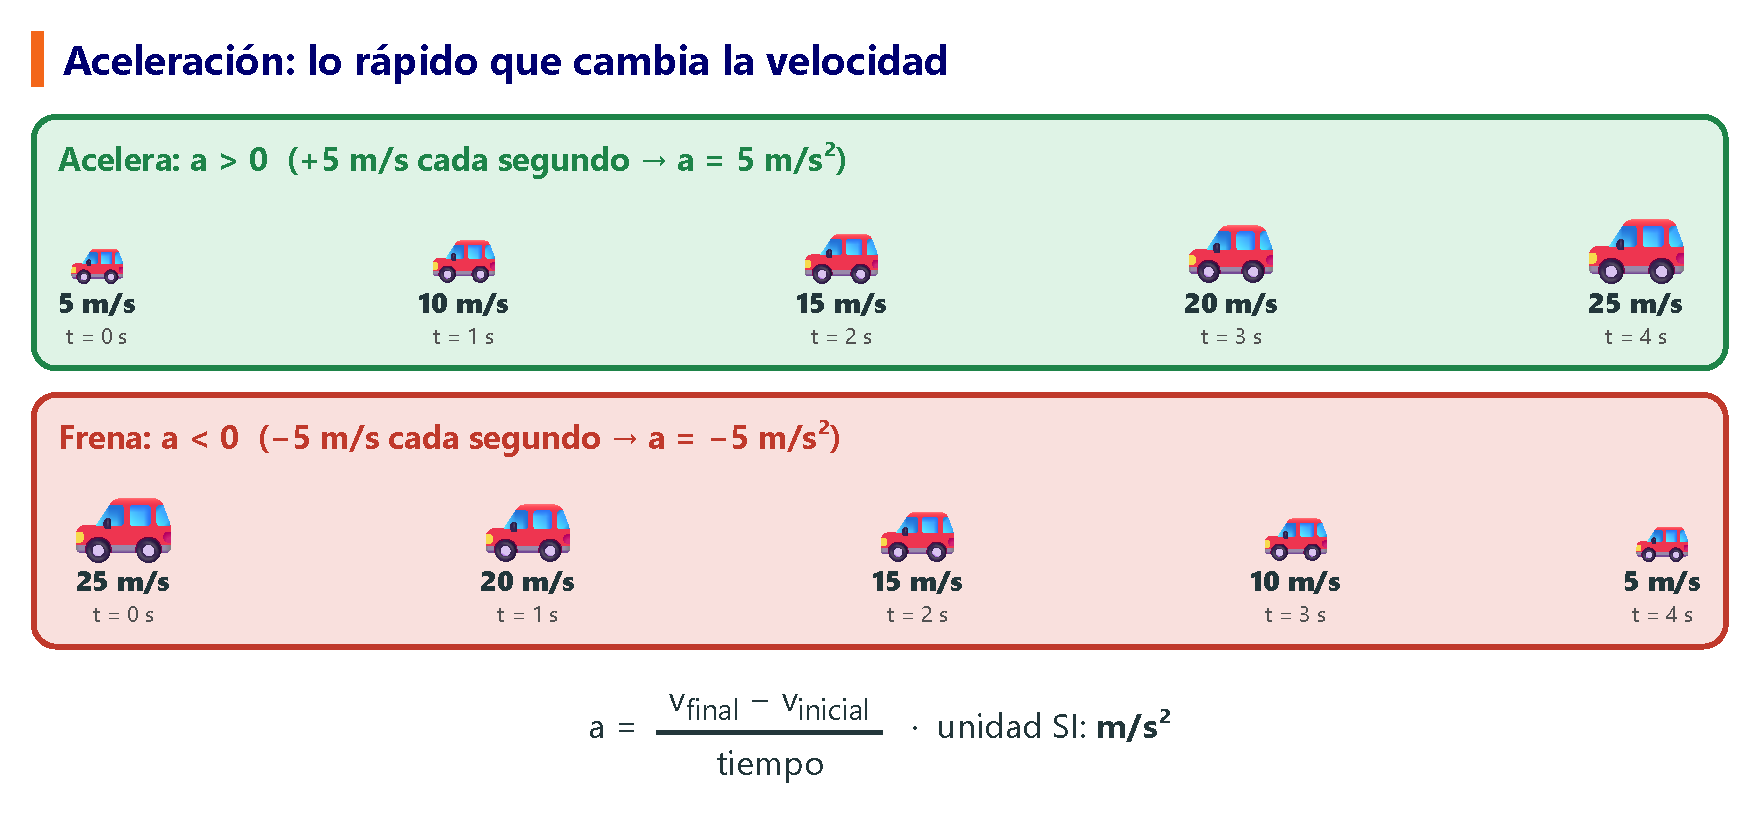
\includegraphics[width=\textwidth]{FigurasSVG/Unit_7_Motion/pdf/acceleration_es.pdf}
    \caption{Aceleración positiva: la velocidad aumenta. Aceleración negativa: la velocidad disminuye.}
    \label{fig:u7_acceleration}
\end{figure}

\begin{itemize}
    \item Si \(a > 0\) (\textbf{positiva}), el móvil acelera (va cada vez más deprisa).
    \item Si \(a < 0\) (\textbf{negativa}), el móvil frena (va cada vez más despacio).
\end{itemize}

\begin{example}
    \textbf{La velocidad de un coche pasa de \qty{5}{\mps} a \qty{25}{\mps} en cuatro segundos. Calcula su aceleración.}
    \begin{equation*}
        a = \dfrac{\qty{25}{\mps} - \qty{5}{\mps}}{\qty{4}{\s}} = \dfrac{\qty{20}{\mps}}{\qty{4}{\s}} = \qty{5}{\mpss}
    \end{equation*}
\end{example}

\begin{exercise}
    Una pelota que rueda a \qty{12}{\mps} frena de manera uniforme y se para al cabo de \qty{6}{\s}.
    \begin{enumerate}[label=\letraminuscula]
        \item Calcula su aceleración.
        \item ¿El signo de la aceleración es el que esperabas? Explícalo.
    \end{enumerate}
    \begin{solu}
        \begin{enumerate}[label=\alph*)]
            \item \(a = \dfrac{0 - \qty{12}{\mps}}{\qty{6}{\s}} = \qty{-2}{\mpss}\).
            \item Sí: la aceleración es \textbf{negativa} porque la pelota está frenando (su velocidad disminuye con el tiempo).
        \end{enumerate}
    \end{solu}
\end{exercise}

\begin{exercise}
    La velocidad de un móvil pasa de \(\qty{-4}{\mps}\) a \(\qty{-12}{\mps}\) en \qty{4}{\s} (una velocidad negativa significa que se mueve hacia el origen).
    \begin{enumerate}[label=\letraminuscula]
        \item Calcula la aceleración.
        \item ¿El móvil va cada vez más deprisa o más despacio? ¿Coincide con el signo de la aceleración que has obtenido en a)?
    \end{enumerate}
    \begin{solu}
        \begin{enumerate}[label=\alph*)]
            \item \(a = \dfrac{\qty{-12}{\mps} - (\qty{-4}{\mps})}{\qty{4}{\s}} = \dfrac{\qty{-8}{\mps}}{\qty{4}{\s}} = \qty{-2}{\mpss}\).
            \item El móvil va \textbf{cada vez más deprisa} (su rapidez pasa de \qty{4}{\mps} a \qty{12}{\mps}), aunque la aceleración sea negativa. Esto muestra que el signo de la aceleración nos indica el \textbf{sentido} en el que cambia la velocidad, y no simplemente si el móvil acelera o frena: aquí la velocidad y la aceleración tienen las dos sentido negativo, así que el móvil va cada vez más deprisa.
        \end{enumerate}
    \end{solu}
\end{exercise}

\subsection{Movimiento rectilíneo uniformemente acelerado (MRUA)}

\begin{definition}[MRUA]
    Es el movimiento de un cuerpo con trayectoria \textbf{recta} y aceleración \textbf{constante} (distinta de cero): su velocidad aumenta, o disminuye, lo mismo cada segundo.
\end{definition}

\begin{itemize}
    \item \negsubro{Gráfica velocidad-tiempo}: siempre es una línea recta. Una recta \textbf{creciente} indica aceleración positiva; una recta \textbf{decreciente}, aceleración negativa. Cuanto más inclinada está la recta, mayor es la aceleración (en valor absoluto).
    \item \negsubro{Distancia recorrida}: a diferencia del MRU, en un MRUA la distancia recorrida en tiempos iguales \textbf{no} es la misma: aumenta si \(a>0\) y disminuye si \(a<0\).
\end{itemize}

\begin{impt}
    \negsubro{Distancia recorrida a partir de una gráfica velocidad-tiempo, en un MRUA}: igual que en el MRU, la distancia recorrida es el \textbf{área} comprendida entre la recta velocidad-tiempo y el eje del tiempo. Cuando el móvil parte del reposo (\(v_0 = 0\)), esa área es un triángulo, así que:
    \begin{equation*}
        \text{distancia} = \dfrac{v_{\text{final}} \cdot t}{2}
    \end{equation*}
\end{impt}

\begin{figure}[H]
    \centering
    % [FIGURA ORIGINAL] \includegraphics[width=\textwidth]{Unit_7/uarm_graphs}
    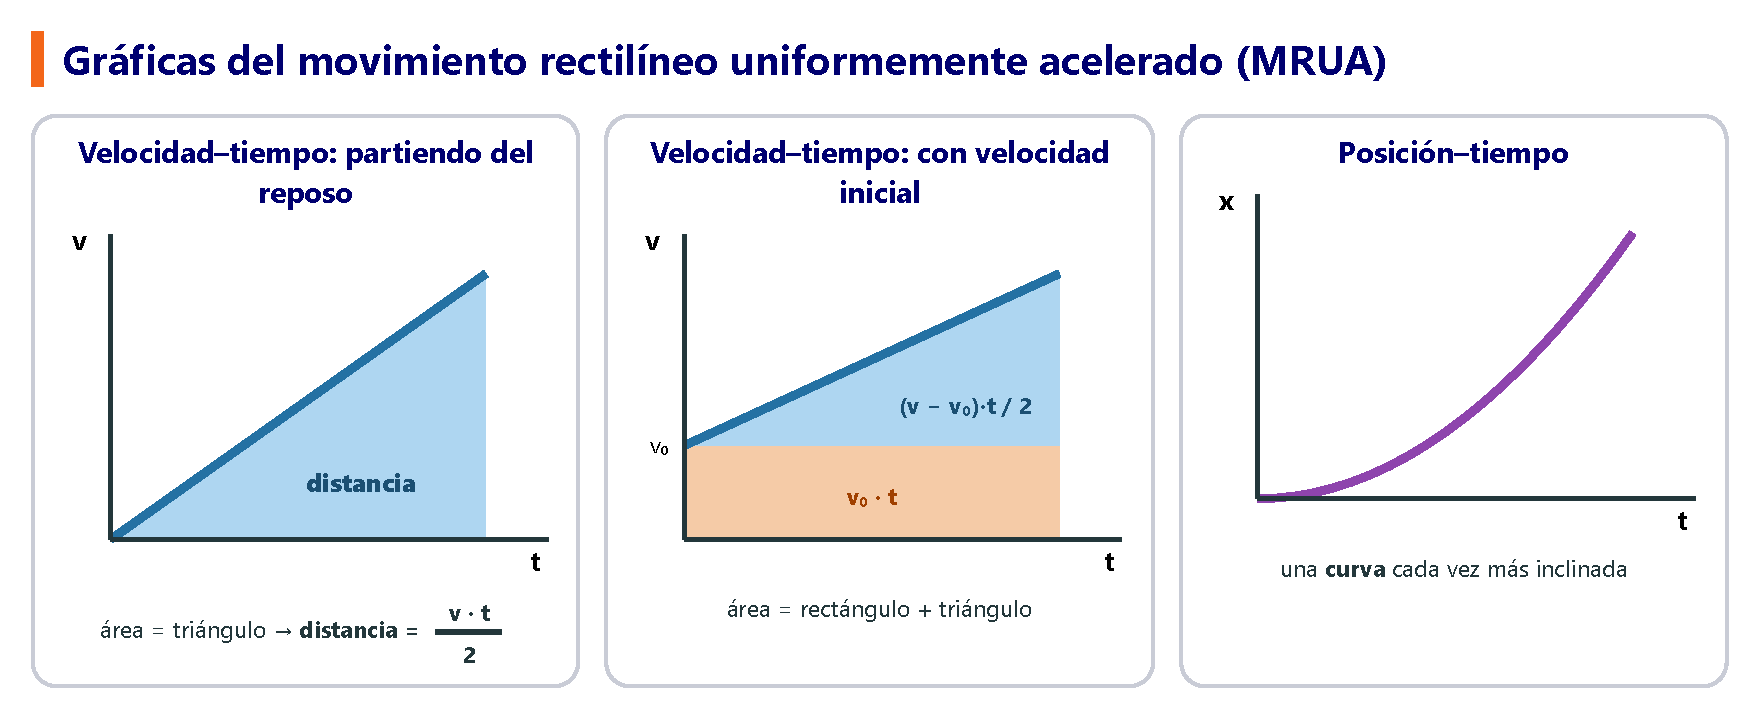
\includegraphics[width=\textwidth]{FigurasSVG/Unit_7_Motion/pdf/uarm_graphs_es.pdf}
    \caption{Gráficas de un MRUA: el área bajo la gráfica velocidad-tiempo es la distancia recorrida.}
    \label{fig:u7_uarm_graphs}
\end{figure}

\begin{example}
    \textbf{Una patinadora parte del reposo y alcanza \qty{6}{\mps} en \qty{4}{\s}, con aceleración constante. Calcula la aceleración y la distancia recorrida.}
    \begin{equation*}
        a = \dfrac{\qty{6}{\mps} - 0}{\qty{4}{\s}} = \qty{1.5}{\mpss}
    \end{equation*}
    La gráfica velocidad-tiempo forma un triángulo (una recta de \((0,0)\) a \((4,6)\)), así que:
    \begin{equation*}
        \text{distancia} = \dfrac{v_{\text{final}} \cdot t}{2} = \dfrac{\qty{6}{\mps} \cdot \qty{4}{\s}}{2} = \qty{12}{\m}
    \end{equation*}
\end{example}

\begin{exercise}
    Un coche va a \qty{5}{\mps} y acelera de manera uniforme hasta \qty{15}{\mps} en \qty{8}{\s}.
    \begin{enumerate}[label=\letraminuscula]
        \item Calcula su aceleración.
        \item El área bajo su gráfica velocidad-tiempo es un trapecio: un rectángulo de altura \(v_0\) más un triángulo de altura \(v_{\text{final}} - v_0\), los dos de base \(t\). Calcula la distancia recorrida.
    \end{enumerate}
    \begin{solu}
        \begin{enumerate}[label=\alph*)]
            \item \(a = \dfrac{\qty{15}{\mps} - \qty{5}{\mps}}{\qty{8}{\s}} = \qty{1.25}{\mpss}\).
            \item Rectángulo: \(v_0 \cdot t = \qty{5}{\mps} \cdot \qty{8}{\s} = \qty{40}{\m}\). \\
            Triángulo: \(\dfrac{(v_{\text{final}}-v_0)\cdot t}{2} = \dfrac{\qty{10}{\mps} \cdot \qty{8}{\s}}{2} = \qty{40}{\m}\). \\
            Distancia total \(= 40 + 40 = \qty{80}{\m}\).
        \end{enumerate}
    \end{solu}
\end{exercise}

\begin{exercise}
    Un carrito parte del reposo con una aceleración constante de \qty{2}{\mpss}.
    \begin{enumerate}[label=\letraminuscula]
        \item Completa una tabla con la velocidad cada segundo, desde \(t=0\) hasta \(t=4\) s.
        \item Calcula la distancia recorrida en esos \qty{4}{\s} con la fórmula del triángulo.
    \end{enumerate}
    \begin{solu}
        \begin{enumerate}[label=\alph*)]
            \item Como \(v = a \cdot t\):
            \begin{center}
                \begin{tabular}{cccccc}
                    \toprule
                    \(t\) (s) & 0 & 1 & 2 & 3 & 4 \\
                    \midrule
                    \(v\) (m/s) & 0 & 2 & 4 & 6 & 8 \\
                    \bottomrule
                \end{tabular}
            \end{center}
            \item \(\text{distancia} = \dfrac{v_{\text{final}} \cdot t}{2} = \dfrac{\qty{8}{\mps} \cdot \qty{4}{\s}}{2} = \qty{16}{\m}\).
        \end{enumerate}
    \end{solu}
\end{exercise}

%----------------------------------------------------------------------------------------

\section*{Resumen}

\begin{itemize}
    \item \textbf{El movimiento es relativo} al sistema de referencia elegido. Magnitudes clave: posición (\(x\)), trayectoria, distancia recorrida y desplazamiento.
    \item \textbf{Velocidad} \(= \) desplazamiento / tiempo (unidad del SI: \unit{\mps}). La velocidad media se calcula con todo el trayecto; la velocidad instantánea se lee en un instante.
    \item \textbf{MRU}: velocidad constante y trayectoria recta; la gráfica posición-tiempo es una recta; la gráfica velocidad-tiempo es una recta horizontal; distancia = área bajo la gráfica velocidad-tiempo.
    \item \textbf{Aceleración} \(=\) variación de la velocidad / tiempo (unidad del SI: \unit{\mpss}). \textbf{MRUA}: aceleración constante y trayectoria recta; la distancia recorrida en tiempos iguales cambia; distancia = área bajo la gráfica velocidad-tiempo (un triángulo, si parte del reposo).
\end{itemize}

\section{Vocabulario}

\begin{vocabulary}[Sistema de referencia (\textit{frame of reference})]
    Punto, o conjunto de puntos, fijo que se usa para describir la posición y el movimiento de un cuerpo.
\end{vocabulary}

\begin{vocabulary}[Trayectoria (\textit{trajectory})]
    Línea que sigue un móvil.
\end{vocabulary}

\begin{vocabulary}[Desplazamiento (\textit{displacement})]
    Distancia más corta entre la posición inicial y la posición final de un móvil.
\end{vocabulary}

\begin{vocabulary}[Velocidad (\textit{speed, velocity})]
    Magnitud que mide lo deprisa que se mueve un cuerpo; distancia recorrida por unidad de tiempo.
\end{vocabulary}

\begin{vocabulary}[Aceleración (\textit{acceleration})]
    Magnitud que mide la variación de la velocidad por unidad de tiempo.
\end{vocabulary}

\begin{vocabulary}[Movimiento rectilíneo uniforme (\textit{uniform rectilinear motion})]
    Movimiento con trayectoria recta y velocidad constante.
\end{vocabulary}

\begin{vocabulary}[Movimiento rectilíneo uniformemente acelerado (\textit{uniformly accelerated rectilinear motion})]
    Movimiento con trayectoria recta y aceleración constante.
\end{vocabulary}
